\section{The Proposed Method -GAN Segmentation Method}
\label{segmethod}


The GAN network image generation and the blood object segmentation process consist of the following components: blood smears image acquisition, image generation with GANs networks (Figure \ref{fig:maincomp} ),  apply adaptive  threshold filter () and image segmentation.



\begin{figure*}[h]
\label{fig:maincomp}
  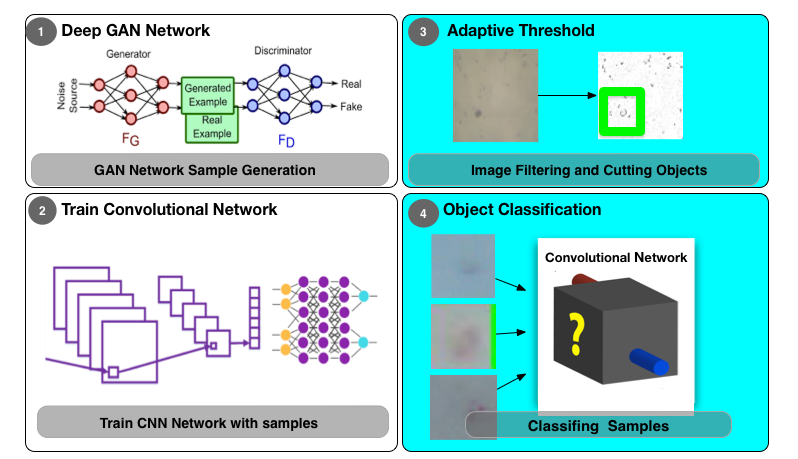
\includegraphics[width=\textwidth]{images/MainComponents.png}
  \caption{Main components of the proposed method .}
\end{figure*}



\begin{figure}[h]
\label{fig:gen50}
\begin{center}
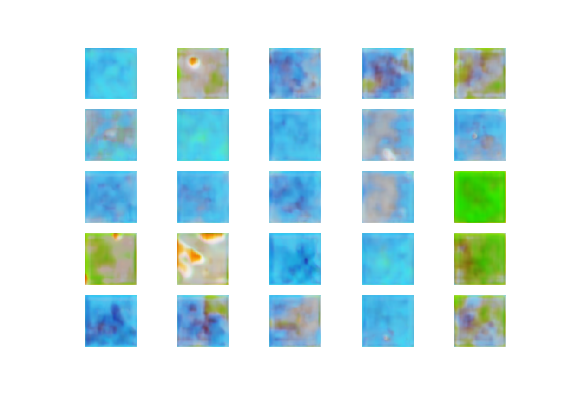
\includegraphics[scale=0.45]{./images/generation/alta_mnist_50.png} \end{center}
\caption{Generated images after 50 epochs}
\end{figure}

\begin{figure}[h]
\label{fig:gen250}
\begin{center}
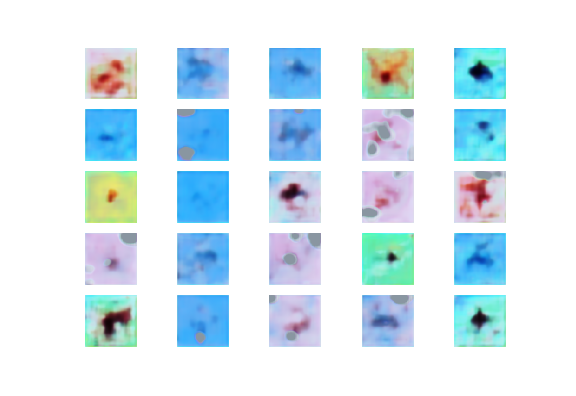
\includegraphics[scale=0.45]{./images/generation/alta_mnist_250.png} \end{center}
\caption{Generated images after 250 epochs}
\end{figure}


\begin{figure}[h]
\label{fig:gen250}
\begin{center}
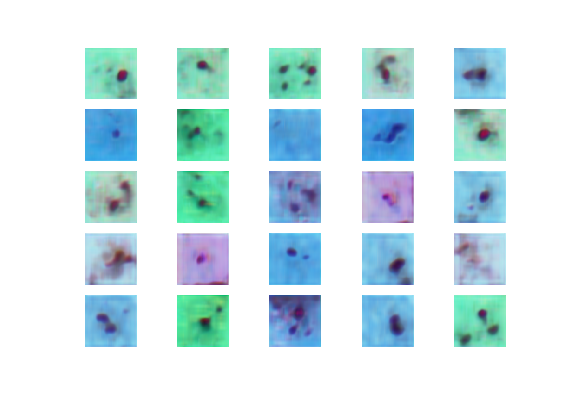
\includegraphics[scale=0.45]{./images/generation/alta_mnist_30410.png} \end{center}
\caption{Generated images after 30410 epochs}
\end{figure}


\begin{figure}[h]
\label{fig:gen250}
\begin{center}
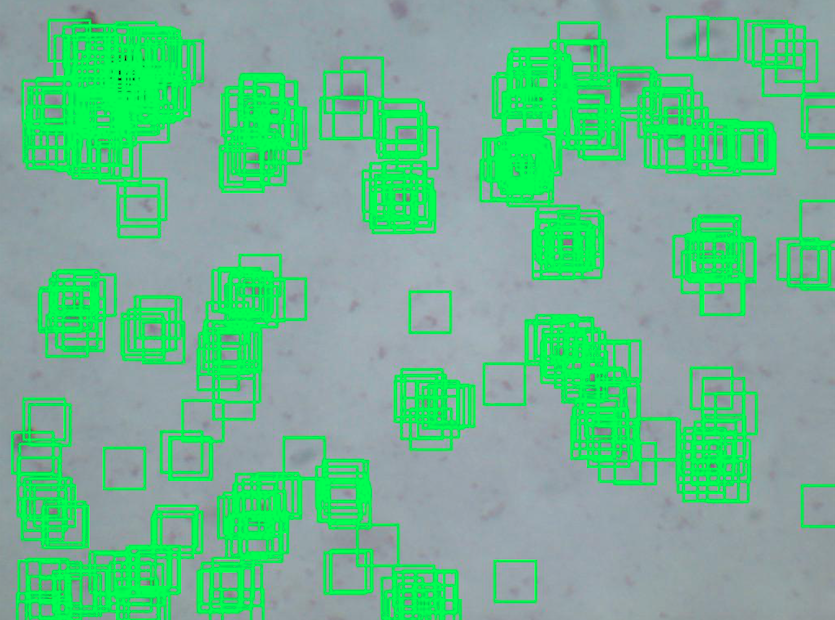
\includegraphics[scale=0.45]{./images/object_detected.png}

\end{center}
\caption{Generated images after 30410 epochs}
\end{figure}


\begin{figure}[h]
\label{fig:gen250}
\begin{center}
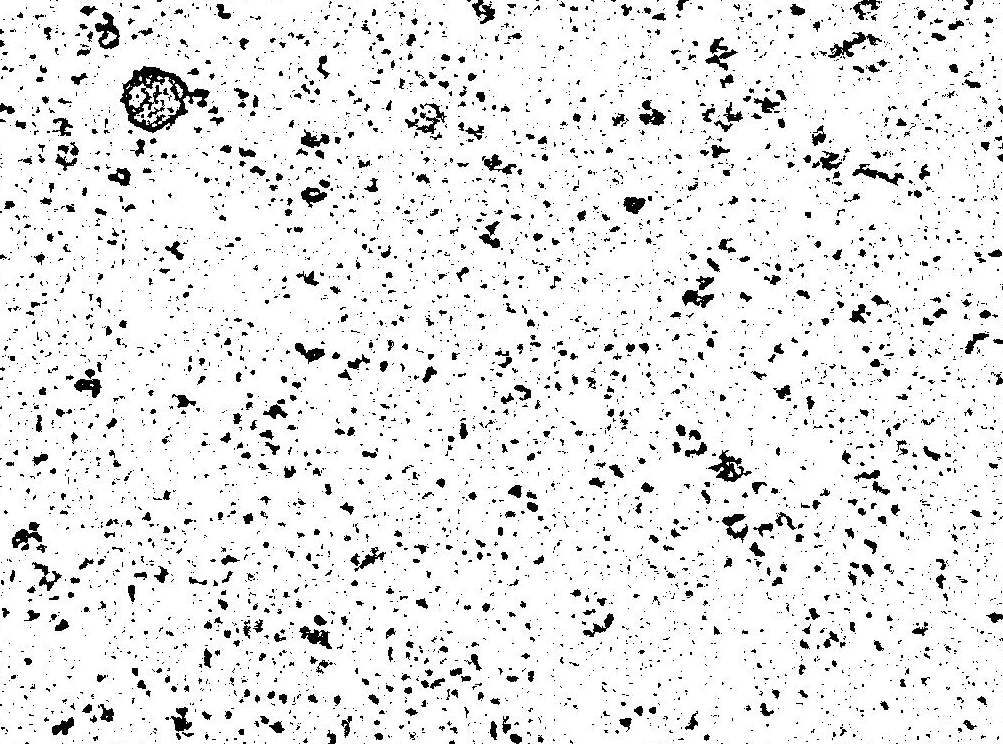
\includegraphics[scale=0.45]{./images/threshold.png}

\end{center}
\caption{Generated images after 30410 epochs}
\end{figure}

% Please add the following required packages to your document preamble:
% \usepackage[table,xcdraw]{xcolor}
% If you use beamer only pass "xcolor=table" option, i.e. \documentclass[xcolor=table]{beamer}
\begin{table}[h]
\caption{Results of training the CNN network with images generates by DGAN network}
\label{tab:results}
\begin{tabular}{|l|l|l|l|}
\hline
\rowcolor[HTML]{C0C0C0} 
\textbf{\begin{tabular}[c]{@{}l@{}}Number of \\ Samples \\ Created\\ by GAN \\ Network\end{tabular}} & \textbf{\begin{tabular}[c]{@{}l@{}}Number of\\ Real \\ Images\\ for Test\end{tabular}} & \textbf{\begin{tabular}[c]{@{}l@{}}Number \\ of correctly \\ classified \\ samples\end{tabular}} & \textbf{\begin{tabular}[c]{@{}l@{}}Number of \\ incorrectly \\ classified \\ samples\end{tabular}} \\ \hline
600                                                                                            & 600                                                                                 & 420 (70 \%)                                                                                      & 180                                                                                                \\ \hline
800                                                                                            & 600                                                                                 & 406 (68 \%)                                                                                      & 194                                                                                                \\ \hline
1000                                                                                           & 600                                                                                 & 453 (76 \%)                                                                                      & 147                                                                                                \\ \hline
1200                                                                                           & 600                                                                                 & 424 (71 \%)                                                                                      & 176                                                                                                \\ \hline
1400                                                                                           & 600                                                                                 & \begin{tabular}[c]{@{}l@{}}429 \\ ($\sim$71 \%)\end{tabular}                                     & 171                                                                                                \\ \hline
1600                                                                                           & 600                                                                                 & 430 (72 \%)                                                                                      & 170                                                                                                \\ \hline
1800                                                                                           & 600                                                                                 & 480 (80  \%)                                                                                     & 120                                                                                                \\ \hline
2200                                                                                           & 600                                                                                 & 600 (100 \%)                                                                                     & 0                                                                                                  \\ \hline
\end{tabular}
\end{table}

